\documentclass[titlepage, 12pt]{extarticle}
\usepackage[margin=1in]{geometry}
\usepackage{tikz}
\usepackage{tikz-uml}
\usepackage{fancyhdr}
\usepackage{lastpage}

\lhead{Inf2C: SE Coursework 1}
\rhead{s1703773 \& s1737075}
\cfoot{\thepage~/~\pageref{LastPage}}
\pagestyle{fancy}
\begin{document}
\title{{\bf Inf2C: Software Engineering \\Coursework 2 \vspace{2em}\\ Creating a software design for an auction house system}}
\author{
\begin{tabular}{l  c}
  Michael Andrejczuk & s1703773 \\
  Dylan Joseph Thinnes & s1737075
\end{tabular}
}
\date{November 5, 2018}
\maketitle

\tableofcontents
\newpage

\section{Introduction}
We provide a software design for an auction house system, codenamed Auctionista. Our design is consistent with the requirements design undertaken in Coursework 1. We provide UML class models for the key actors involved in the system, and sequence diagrams and behavior descriptions for use-cases identified in Coursework 1. For further details, please refer to the specification for Coursework 2.
\newpage
\section{Static model}
\subsection{UML class model}
We begin with a model of classes and their attributes and operations:\\\\
\begin{tikzpicture}
  \umlclass{User}{
  }
  { browseLots(void) : void \\
  }

  \umlclass{Registered user}{details : PersonalDetails \\
    paymentDetails : BankDetails \\
    contactDetails : ContactDetails \\
    username : String \\
  }{
    User(PersonalDetails, BankDetails, ContactDetails, String) : User\\
  }
  
  \umlclass{Buyer}{
    lotsInterestedIn : List \textless Lot\textgreater \\
    lotsBidOn : List \textless Lot\textgreater
    bidList : List \textless Bid\textgreater}
  {
    markInterestInLot(Lot) : boolean \\
    removeInterestInLot(Lot) : boolean \\
    bidOnLot(Lot, Bid) : boolean\\
  }

  \umlclass{Seller}{
    lotsOwned : List \textless Lot\textgreater \\
  }
  {
    addLot(Lot, Auction) : \\
  }

  \umlclass{Auctioneer}{
    lotsAssigned : List \textless Lot\textgreater \\
  }
  {
    openBidding() : \\
    closeBidding() : \\
  }

  \umlclass{Lot}{
    auctionStatus : enum(preAuction, inProgress, postAuction) \\
    seller : Seller \\
    auction : Auction \\
    auctioneer : Auctioneer \\
    startTime : DateTime \\
    description : LotDescription \\
    highEstimate : Money \\
    lowEstimate : Money \\
    reservePrice : Money \\
    minimumBidIncrement : Money \\
    interestedBuyers : List \textless Buyer\textgreater \\
    bidList : List \textless Bid\textgreater \\
    currentPrice : Money \\ 
    finalBid : Bid
  }
  {
    Lot(Money, Money, Money, Money, Seller, Auction) : Lot \\
    % Lot(highEstimate Money, lowEstimate Money, reservePrice Money, \\
    % minimumBidIncrement Money, seller Seller, auction Auction)
    receiveBid(Buyer, Bid) : boolean\\
    openBidding() : boolean \\
    closeBidding() : boolean \\
    setAuctioneer(Auctioneer) : boolean \\
  }

  \umlclass{Auction}{
    lots: List \textless Lot\textgreater \\
    auctioneers: List \textless Lot\textgreater \\
    startTime : DateTime \\
    % auction has guaranteed end time, but a lot may not
    endTime : DateTime \\   
  }{
    % nb. getters and setters are implied
  }

  \umlclass{Bid}{
    lot : Lot \\
    seller : Seller \\
    buyer : Buyer \\
    bidType : enum(Increment, JumpBid) \\
    bidValue : Money
  }{
    Bid(Lot, Seller, Buyer, bidType, bidValue) : Bid \\
  }
\end{tikzpicture}
\newpage
Next we give a picture of associations between classes:\\\\
\begin{tikzpicture}
  % TODO add bid class
  \umlsimpleclass[x=4, y=-6]{Buyer}
  
  \umlsimpleclass[x=0, y=0]{User}

  \umlsimpleclass[x=4, y=-3]{Registered user}

  \umlsimpleclass[x=4, y=0]{Seller}

  \umlsimpleclass[x=9, y=0]{Auctioneer}

  \umlsimpleclass[x=0, y=-3]{Guest user}

  \umlsimpleclass[x=0, y=-6]{Auction house}

  \umlsimpleclass[x=9, y=-3]{Lot}

  \umlsimpleclass[x=12, y=-2]{Auction}

  \umlassoc[mult1=1, mult2=*]{Buyer}{Lot}
  \umlassoc[mult1=1, mult2=*]{Seller}{Lot}
  \umlassoc[mult1=1, mult2=*]{Auction}{Lot}
  \umlassoc[mult1=*, mult2=*]{Auction}{Auctioneer}
  
  \umlinherit{Registered user}{User}
  \umlinherit{Buyer}{Registered user}
  \umlinherit{Seller}{Registered user}
  \umlinherit{Guest user}{User}
\end{tikzpicture}
\newpage
\subsection{High-level description}

\section{Dynamic models}
\subsection{UML sequence diagram}
\subsection{Behaviour descriptions}
\end{document}
